%!TEX root = ThesisLKN.tex
\chapter{Literature Review} \label{chapter:2}

This chapter lists literatures that are related to methods or concepts used in this thesis work. Section \ref{lr:tracking} discusses two classical ways of tracking object and introduces BOF and its variants. Section \ref{lr:dynamic} presents literatures that try to model dynamics in environment. Section \ref{lr:network} details recent researches on neural networks and correlations between RNNs and Bayesian filters. 

\section{Object Tracking} \label{lr:tracking}

Perception of environment can be done with different sensors, which also differentiates object tracking applications. Visual tracking refers to object tracking with RGB cameras \citep{ross2008incremental}. In this thesis work, however, we mainly concern object tracking with 2D laser scanners. One popular paradigm of performing tracking is tracking by detection: moving objects are firstly detected and then determine how to pair them with existing tracks. Generally, there are two approaches to deal with detection based object tracking: \textit{model-free} and \textit{model-based} \citep{wang2015model}. 

The detection of model-free object tracking works based on motion cues. In this case, prior knowledge on neither object's semantic information (whether it is a car or a person) nor object's shape or geometric properties is needed. However, this approach only tracks objects that show instantaneous motion dynamics and potential moving objects might be neglected. BOF can be regraded as a model-free tracking algorithm since it predicts occupancies based on cells' velocities. Similar to BOF, \citet{ross2008incremental} models the environment with occupancy gird map. Their work combines SLAM with dynamic object tracking in outdoor environment. Once the vehicle equipped with laser sensors is self-located and objects are detected by motion cues, they apply a method called Global Nearest Neighborhood (GNN) for tracking. On the contrary, for model-based tracking, semantic class of the objects being tracked is given, and detection is done with the help of a parametric model of the object's shape. For human tracking, a person is represented as point blob or modeled based on detection of legs \citep{arras2008efficient, cui2006laser}. 

The tracking by detection paradigm has to address \textit{data association} explicitly, which is known to be as the main difficulty in tracking. Data associations refers to match detections of moving objects in new observations to a set of tracked trajectories from last time step. To address data association problems in tracking, many methods have been proposed in literature. Historically, nearest neighbors based approaches are used in the early stage \citep{fod2002laser}. \citet{schulz2001tracking} detect people by their legs in 2D laser scans and propose the Joint Probabilistic Data Association Filter (JPDAF) for tracking. \citet{arras2008efficient} is similar in identifying people with legs but their tracking is done with Multi-hypothesis tracking (MHT). Although the mentioned methods partially address the data association problem, their performance is not stable in densely cluttered environments, where occlusions happen quite often.

On the contrary to tracking by detection paradigm, tracking can also be done without detection, e.g., tracking by filtering. \citet{coue2006bayesian} propose Bayesian Occupancy Filter for object tracking in automotive applications. The environment is represented by a grid map, and the state of each cell is characterized by its occupancy and velocity. Inspired by Bayesian Filter, tracking works in a form of recursive \textit{predictions} and \textit{estimations} of cell's state. One of important advantages of BOF is that the concepts of \textit{objects} and \textit{tracks} are replaced by transitions of occupancies between cells over time. That is to say, data association is addressed implicitly by BOF. Later works extend BOF to better adapt to real world situations. BOF's linear motion model cannot adapt to traffic scenarios like curved roads. Therefore, \citet{gindele2009bayesian} propose to enrich motion model of BOF with prior map knowledge (BOFUM), which can be obtained from navigation systems. By this way, BOFUM predicts occupancies according to motion preferences at different locations, which results in reliable estimates even when occlusion happens. 

Despite of various variants of BOF, all of them assume that objects perform linear motion. However, linear motion is obviously over-simplified for real world scenarios. Besides, since objects cannot appear or disappear suddenly, the state changes of a cell's neighboring cells contain valuable information for prediction of its future state. Therefore, we proposed to model human motion patterns in a way that captures both place dependency and spatial correlation of cells. This motion model is then incorporated into BOF framework to perform human tracking. A similar idea is used in the work of \citet{luber2011place}, which proposed a place dependent people tracking algorithm. Unlike BOF which tracks objects by filtering, they perform people tracking by detection and data association. They proposed to model human activity events as a three-layer spatial affordance map with each layer characterizing the probability distribution of new tracks, matched tracks and false alarms respectively. Each layer is represented by a \textit{spatial} Poisson process which introduces spatial dependency and the parameter of each cell is learned from a sequence of observations. Figure \ref{fig:affordance} shows one example of two layers of the learned spatial affordance map. Their motion model is place dependent because it is dependent on the spatial affordance map. They use boosted features for people detection \citep{arras2007using} and they extend multiple hypothesis tracking (MHT) for data association. Their results show they achieve more accurate tracking behavior in terms of data association errors. 

\begin{figure}[H]
  \centering
    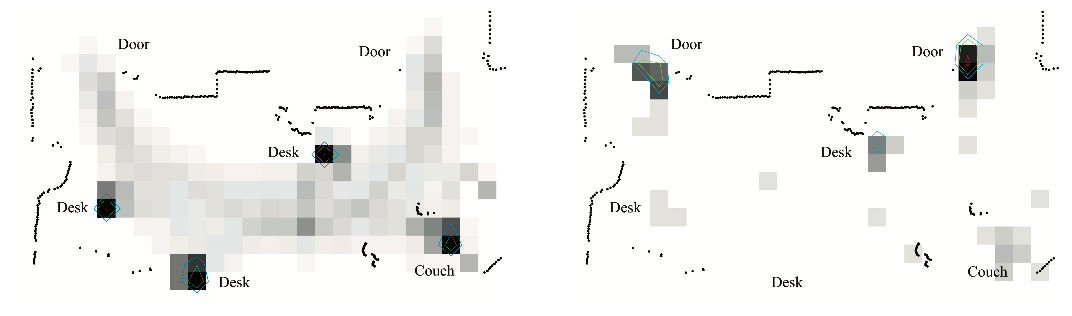
\includegraphics[width=\textwidth]{figures/affordance_map.png}
    \caption[Two layers of a spatial affordance map.]{Two layers of a learned spatial affordance map \citep{luber2011place}. On the left shows probability distribution of matched track events, and on the right shows that of new track events. Note that the maxima show at different regions in two maps. While on the left the maxima appear at places frequently used by people (desks and coach), on the right the maxima of new track events indicate places where people normally appear from, i.e., doors, desks and coach.}
    \label{fig:affordance}
\end{figure}

\section{Dynamics Modeling} \label{lr:dynamic}

Nowadays, more and more robots are entering \textit{dynamic} environments. In order to fulfill their task, it is imperative for robots to understand these dynamics. In the context of human tracking, these dynamics refer to human movements in the environment. In literature, some researchers try to model human dynamics explicitly by a motion model. Meanwhile, others model them implicitly by regarding human dynamics as part of the environment and therefore model the environment directly. We discuss dynamics modeling separately according to these two approaches. In both cases, we represent the environment as a gird map with each cell representing a possible location. 

\subsection{Human Motion Modeling}

In the early stage of human tracking, researches adopts simple and conservative motion models. \citet{montemerlo2002conditional} uses Brownian motion model for human tracking with Bayesian filters.  The Brownian motion assumes people take random directions at each time step and there is no dependence between time steps. In other words, Brownian motion does not assign human dynamics with any pattern other than dispersion. As a consequence, when there is no observations, the predictions of people locations spread out over a large area very quickly. This is a poor estimate as we know people normally does not move randomly. In reality, people normally go from the starting point and follow some motion patterns until they reach destination. A more realistic model is the first order motion model (a.k.a. linear motion model). For example, \citet{meier1999using} used this model together with Kalman filter for human tracking. First order motion model assumes people always move in the same direction as in the last time step. This assumption might be true if a person is walking along a straight corridor, but in many cases it is invalid because people often need to make turns around corners. Some researchers proposed better ways to model people motion patterns. For example, \citet{bruce2004better} learns destinations by clustering real trajectories and uses a path planer to those destinations as a reference for human motion patterns. \citet{liao2003voronoi} assumes that human tend to move along Voronoi graph of the environment and therefore constraint motion patterns by Voronoi graph. 

Our motion model is different to above methods in two aspects: fineness and cell dependency. The Voronoi graph is constructed based on a \textit{global} representation of the environment. It is predefined and only well suited for applications where high-level motion clue is needed (e.g., which rooms a person has visited). This kind of motion clues are too less precise to be used for recovering a person's exact location. Therefore, in order to get a finer motion model, we decompose the \textit{global} task of modeling human motion pattern into \textit{local} tasks at \textit{cell level}. On the other hand, although a path planer to the learned destination defines an effective path, it does not necessarily cover the motion dynamics at every possible locations and assumes no dependency between these locations. One intuition we captured based on observations of human motion is that, for a cell in the map, the state changes of its neighboring cells is a strong indicator of predictions of its future state. To capture this \textit{spatial} correlation, we propose to model changes of movement directions. For each cell, we learn based on human trajectories how likely a person's moving direction changes for the next time step, conditioned on the direction with which he or she enters this cell. Moreover, this way of motion modeling also captures \textit{temporal} correlations, since it builds connections for each cell with its neighboring cells from both last time step and next time step. 

In fact, after we came up with above way of modeling human motion, we found in literature the same idea has been used by \citet{kucner2013conditional} in an autonomous navigation scenario. Their model, which is named as Conditional Transition Map, is created by ``learning the probability distribution of an object leaving to a certain neighboring cell, given the cell from which it entered into the current cell.'' They demonstrate their method with a roundabout, and the corresponding model is illustrated in Figure \ref{fig:condi_tran_map}. One can see that at different locations in the roundabout, different motions are learned, which accurately models how cars drive through the roundabout. The difference between our method and theirs lies in how those probabilities are learned. The cross-correlation of temporal occupancy signals extracted from observations is used for learning in their method, while our model learns these probabilities by training a neural network. With lots of different maps as training data, our network is able to learn the motion patterns that are constrained by spatial structures of these maps. One of the most important advantages of our method is that our network can generalize motion patterns for maps that never occur in training data. Therefore, our method can work in new environments without learning these probabilities from scratch. 

\begin{figure}[H]
  \centering
    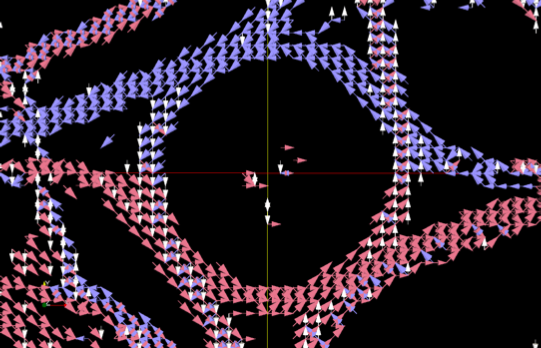
\includegraphics[width=.6\textwidth]{figures/condi_tran_map.png}
    \caption[Conditional transition map of a roundabout.]{Conditional transition map of a roundabout \citep{kucner2013conditional}. Arrows indicate the exit directions for that cell. For simplicity, the entering directions are not drawn. One can see that this model captures how cars drive through the roundabout. }
    \label{fig:condi_tran_map}
\end{figure} 

\subsection{Dynamic Environment Modeling}

For a mobile robot to operate, a proper way to model the environment is necessary. \citet{elfes1989using} introduces occupancy grid as a representation of environment, which divides the environment into a grid of cells with a predefined resolution. Each cell is a random variable with values of either \textit{occupied} or \textit{not occupied}. The occupancy grid assumes the environment being static, which does not hold in real world situations. For example, a robot might need to work in a traffic intense environment with driving cars and pedestrian. 

Early attempts to model dynamics in environment extents occupancy gird with a timescale framework. \citet{arbuckle2002temporal} propose to model dynamics with a stack multiple occupancy grids with each layer corresponding to a different timescale. They call this representation as Temporal Occupancy Grid (TOG). Objects' motion pattern can then be classified based on objects' occupancy traces across different layers of TOG. For example, if a cell is occupied across all layers of TOG (i.e., occupied at all timescales), it is likely to be part of background. Similarly, traffic patterns with various speeds can be identified based on its occupancy traces on a certain layer of TOG. \citet{biber2009experimental} uses multiple map representations of the dynamic environment with different timescales for long-term SLAM. Updates of mapping is calculated based on a (dynamic) sample set of observations that is updated over time by random replacement. Different timescales correspond to different learning rate. Map with higher learning rate adapts to new observations faster than these with lower learning rates.

Although the above methods can be applied for modeling dynamics, essentially their static nature remains if we look at each layer that characterizes a specific timescale. In order to capture the dynamic nature of environment, \citet{meyer2012occupancy} propose to model state changes of cells by a two-state hidden Markov models (HMMs). Therefore, the dynamics in environments are explicitly characterized by the state transition probabilities of HMMs. The parameters of these HMMs are estimated with an Expectation Maximization (EM) algorithm. 

However, although their method relaxes the static cell state assumption made by occupancy grid, they assume that state changes of cells are caused by a \textit{stationary} process, i.e., cell's state transition probabilities are constants over time. Moreover, the assumption of independences between cells is not always valid (e.g., state changes of a cell's neighboring cells are strong indicators of that cell's future state because objects normally move in a continuous manner). Due to above reasons, cell-specific input-output HMMs (IOHMMs) are used by \citet{wang2014modeling} to better model dynamic environments. An IOHMM imposes conditional dependences on latent variables and observed variables with an input sequence. An illustration of IOHMM used in their method is depicted in Figure \ref{fig:IOHMM}. The input sequence is determined by past observations in neighboring cells. By this way, the transition model of their method is adaptive to input sequence that varies over time, which relaxes the assumption of stationary process made by \citet{meyer2012occupancy}. It also incorporates spatial correlations by making input sequence dependent on neighboring cells. 

\begin{figure}[H]
  \centering
    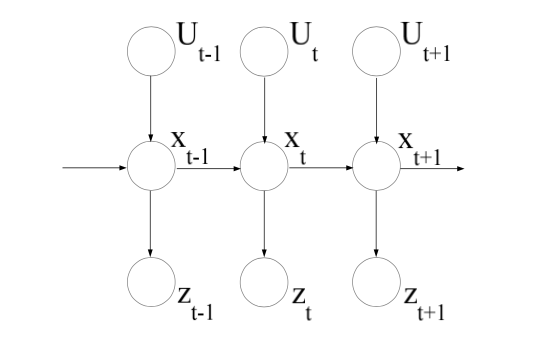
\includegraphics[width=.6\textwidth]{figures/IOHMM.png}
    \caption[An illustration of IOHMM.]{An illustration of IOHMM used by \citet{wang2014modeling}. Note in this IOHMM only latent variables are dependent on input sequence, which is determined by past events in neighboring cells.}
    \label{fig:IOHMM}
\end{figure} 

Our method is conceptually equivalent to theirs. In both methods, the influence of neighboring cells is captured by conditional dependence. Although our motion model is fixed for a specific map, the occupancies propagate to a certain cell only when its neighboring cells have velocities towards it. This mechanism acts as a ``trigger'' which only get triggered at certain time and essentially makes our model time dependent.


\section{Neural Networks} \label{lr:network}

Since \citet{krizhevsky2012imagenet} applied deep convolutional neural networks (CNNs) in large scale image classification from 2012, CNNs have gained a lot of successes in computer vision. Researches show that the depth of network plays a very important role in CNNs' performance \citep{simonyan2014very}. However, deep networks are more difficult to train, possibly due to poor gradient flow during back-propagation. To address this problem, \citet{he2016deep} propose to fit a \textit{residual} mapping with stacked layers of CNNs instead of fitting the desired underlying mapping directly. This idea is implemented as ``shortcut connections'' between layers, which branches from one layer and connects to one of the followed layers. Moreover, \citet{huang2016densely} extends the idea of residual learning so that each layer has a shortcut connection to every other layer in the network. This design guarantees layers with easy access to its preceding layers and makes feature reuse very easy. Figure \ref{fig:dense_net} shows a five layer densely connected CNN (DenseNet).  Compared with other CNN structures like ResNets, DenseNets are even better at alleviating vanishing-gradient problem and therefore improve classification accuracy with even fewer parameters. 

\begin{figure}[H]
  \centering
    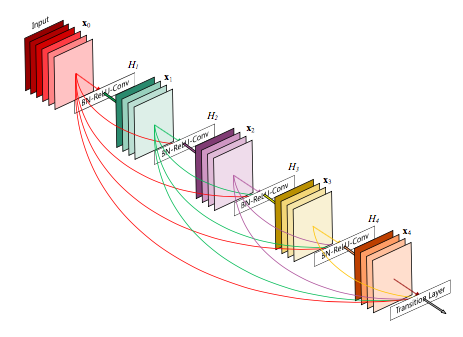
\includegraphics[width=.6\textwidth]{figures/denseNet.png}
    \caption[A five layer dense block.]{A five layer dense block \citet{huang2016densely}. As can be seen, each layer has a shortcut connection to every other follower layer in the network.}
    \label{fig:dense_net}
\end{figure} 

Besides image classification, CNNs have been extensively used in other computer vision tasks like semantic segmentation. Unlike in image classification where only one class has to be determined for the whole image, semantic segmentation requires  classification at pixel level. \textit{Fully} convolutional neural networks have been proposed by \cite{long2015fully} to tackle this problem. By removing fully connected layers and adding a deconvolution layer that functions as upsampling, their network is able to take arbitrary size image as input and predicts pixel-wise classification. Their network also includes skip connections that combine deep coarse features (e.g., semantic information) and shallow fine features (e.g., geometric structure and appearance), both of which are essential for semantic segmentation. \citet{jegou2017one} extends fully convolutional networks with dense blocks, i.e., a block of convolutional layers that \textit{densely} connected as in DenseNet. Their proposed structure is designed for semantic segmentation, with a downsampling path extracting high-level semantic feature and an upsampling path recovering outputs to full resolution as input image. 

The network structure used in this thesis is similar to that of \citet{jegou2017one}. Since our proposed motion model needs to be place dependent, our network is required to predict probabilities at cell level, similar to pixel level prediction in semantic segmentation. The differences lie in the meaning of these probability outputs. For semantic segmentation, these are probabilities of a pixel belonging to a specific semantic class, while in our case they are probabilities of object's exiting direction conditioned on which direction it takes to reach current cell.   

As CNNs are good fit for image based tasks, recurrent neural networks (RNNs) are found to be very useful to deal with sequential data such as videos and texts. RNNs have been successfully applied in applications like object tracking \citep{ondruska2016deep}, automatic language translation \citep{cho2014learning} and speech recognition\citep{graves2013speech}. Long short-term memory (LTSM) \citep{hochreiter1997long} addresses vanishing and exploding gradient problems and becomes one of most popular variants of RNNs. 

\begin{figure}[ht]
  \centering
    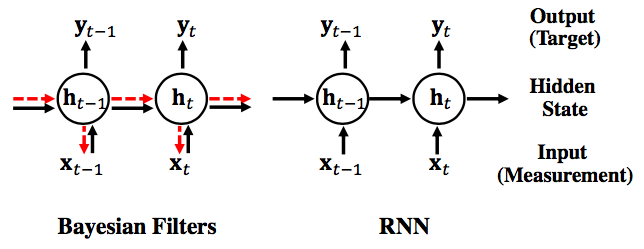
\includegraphics[width=.7\textwidth]{figures/rnn_and_bayes.png}
    \caption[Comparison between RNN and Bayesian filters.]{Comparison between RNN and Bayesian filters \citep{de2017dynamic}. For Bayesian filers, the dynamics are modeled by a Markov process (red dash lines). In both cases, measurements are fed into the systems as inputs.}
    \label{fig:rnn_and_bayes}
\end{figure} 

\citet{ondruska2016deep} propose a framework named as \textit{deep tracking} for object tracking with 2D laser data. Deep tracking uses RNNs as the underlying model, and it is designed to be trained in an end-to-end fashion from raw sensor data without hand-crafted feature engineering. Unlike in most supervised learning applications where human annotated ground truth is needed, they train the network with future sensor observations (i.e., future inputs to network) as ground truth, which essentially makes the training unsupervised. Further, \citet{ondruska2016end} extends their deep tracking framework so that it can perform object tracking and semantic segmentation at the same time. 

The fact that object tracking can be achieved by both Bayesian filter based approaches like BOF and RNN based approaches like deep tracking leads us to understand their connections. In a paper that aims at dynamic facial analysis, \citet{de2017dynamic} try to compare Bayesian filters with RNNs as depicted in Figure \ref{fig:rnn_and_bayes}. Given noisy measurement as input, the goal of Bayesian filter is to estimate the hidden state and optionally the target output, while RNNs sequentially predict target output as a function of hidden state which is in turn dependent on new measurements. The performance of Bayesian filters is highly dependent on how much are the assumed state transition and measurement model close to real situations. While for RNNs, this step of handcrafted engineering is avoided since RNNs are able to model them implicitly by learning from data, which is similar to how CNNs extract features from images without artificial feature engineering. On the other hand, despite its successes in many applications, how the hidden states involve over time and how to interpret the hidden states remain a challenge in understanding RNNs. For Bayesian filter, interpretations of the transition processes are usually quite straightforward. 

